\documentclass[../../../include/open-logic-section]{subfiles}

\begin{document}

\olfileid{sth}{ordinals}{idea}	
\olsection{د ترتيبي عدد عمومي تصور}

طبيعي عددونه په خپل معمولي ترتيب کښې په پام کښې ونيسئ:
\begin{center}
	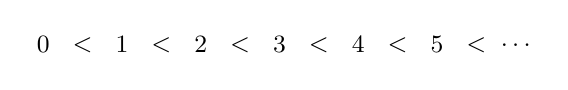
\begin{tikzpicture}
	\foreach \x/\xtext in {0, 1, 2, 3, 4, 5}
	{
		\node (\x a) at (\x, 1) {\small{$\x$}};
		\node (\x a) at (\x.5, 1) {\small{$<$}};
	}
	\node (ldots) at (6, 1) {\small{$\ldots$}};
	\end{tikzpicture}
\end{center}
دې ته په اصطلاحي ژبه کښې $\omega$-لړۍ وايو. او په رښتيا هم
دا عمومي ترتيب زموږ د سټونو د مراتبو د پړاوونو په لومړني جوړښت
کښې څرګندېږي. خو اوس فرض کړئ چې $0$ د دې لړۍ پاے ته يوسو،
داسې چې له نورو ټولو عددونو وروسته راشي:
\begin{center}
	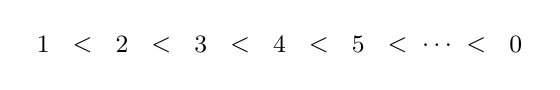
\begin{tikzpicture}
	\foreach \x/\xtext in {1, 2, 3, 4, 5}
	{
		\node (\x a) at (\x, 1) {\small{$\x$}};
		\node (\x a) at (\x.5, 1) {\small{$<$}};
	}
	\node (ldots) at (6, 1) {\small{$\ldots$}};
	\node (bea) at (6.5, 1) {\small{$<$}};
	\node (noa) at (7, 1) {\small{$0$}};
	\end{tikzpicture}
\end{center}
دلته هماغه شيان لرو، خو په بنسټيز ډول بل شان مرتب دي: زموږ
لومړني ترتيب وروستے غړے نۀ لرلو؛ نوے ترتيب ئې لري. په رښتيا
نوے ترتيب د شيانو له يوې $\omega$-لړۍ ($1, 2, 3, 4, 5, \ldots$)
څخه جوړ دے چې ورپسې يو بل شے راځي. دا به $\omega+1$-لړۍ وي.

يوازې د همدې شيانو په کارولو سره د ترتيب نور ډولونه هم جوړولے
شو. مثلاً ټول جفت عددونه (په خپل طبيعي ترتيب کښې) په پام کښې
ونيسئ، او ورپسې ټول طاق عددونه (په خپل طبيعي ترتيب کښې):
\begin{center}
	\begin{tikzpicture}
	\node(a1) at (1,1) {\small{$0$}};
	\node(a2) at (1.5,1) {\small{$<$}};
	\node(a3) at (2,1) {\small{$2$}};
	\node(a4) at (2.5,1) {\small{$<$}};
	\node(a5) at (3,1) {\small{$4$}};
	\node(a6) at (3.5,1) {\small{$<$}};
	\node(dots) at (4,1) {\small{$\ldots$}};
	\node(aaoe) at (4.5,1) {\small{$<$}};
	\node(b1) at (5,1) {\small{$1$}};
	\node(b2) at (5.5,1) {\small{$<$}};
	\node(b3) at (6,1) {\small{$3$}};
	\node(b4) at (6.5,1) {\small{$<$}};
	\node(b5) at (7,1) {\small{$\ldots$}};
	\end{tikzpicture}
\end{center}
دا يوه $\omega$-لړۍ ده چې ورپسې بله $\omega$-لړۍ راځي؛ يعنې
يوه $\omega+\omega$-لړۍ. 

همدغه شان نور هم مخته تللے شو. خو داسې يوه عمومي لاره غواړو
چې د \emph{ترتيبونو} په اړه دا خبرې پرې درک کړو. 

\end{document}
